 \documentclass[border=3pt,tikz]{standalone}
 \usepackage[utf8]{vietnam}
 \usetikzlibrary{calc,angles,intersections,shapes.geometric,arrows,decorations.markings,arrows.meta,patterns.meta,patterns}
 \usepackage{tikz-3dplot,pgfplots}
 \pgfplotsset{compat=1.15}
 \usepgfplotslibrary{polar}
 \usepackage{amsmath}
 \begin{document}
 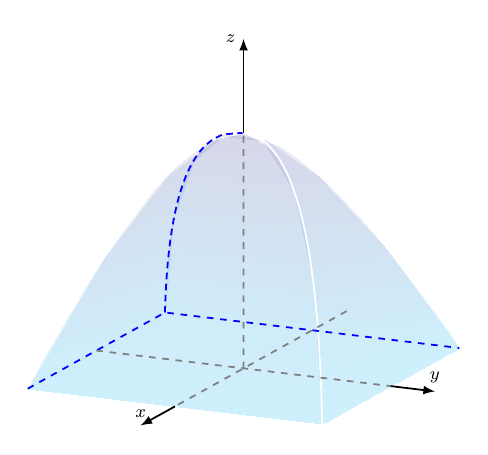
\begin{tikzpicture}[scale=0.8]
	\begin{axis} [hide axis,axis equal, view={115}{15},colormap={mau}{color(0)=(cyan) color(1)=(blue)},z post scale=1.5,shader=interp]
		\addplot3[surf,blue,opacity=0.1,domain=0:1,y domain=-1:1,samples = 22, samples y=8,] ({x},{y*sqrt(x)},{1-x}); % mặt z=1-x 
		\addplot3[surf,blue,opacity=0.1,domain=-1:0,y domain=-1:1,samples = 22, samples y=8,] ({x},{y*sqrt(-x)},{1+x}); % mặt z=1+x
		\addplot3[surf,blue,opacity=0.1,domain=-1:1,y domain=-1:1,samples = 22, samples y=8,] ({x*y^2},{y},{1-y^2}); % mặt z=1-y^2
		\addplot3[surf,blue,opacity=0.1,domain=-1:1,y domain=-1:1,samples = 22, samples y=8,] ({x},{y},{0}); % mặt z=0
		\addplot3[domain=0:1, samples=50, samples y=0, no marks, smooth, thick, white]({x},{sqrt(x)},{1-x});
		\addplot3+[domain=-1:0, samples=50, samples y=0, no marks, smooth, thick, blue]({x},{-sqrt(-x)},{1+x});
		\draw[blue,dashed,thick] (1,-1,0)--(-1,-1,0)--(-1,1,0); 
		\draw[gray,dashed,thick] (-1.5,0,0)--(1,0,0) (0,-1,0)--(0,1,0) (0,0,0)--(0,0,1);
		\draw[-latex,thick] (1,0,0)--(1.5,0,0)node[above]{\footnotesize $x$};
		\draw[-latex,thick] (0,1,0)--(0,1.3,0)node[above]{\footnotesize $y$};
		\draw[-latex,thick] (0,0,1)--(0,0,1.4)node[left]{\footnotesize $z$};
	\end{axis}
\end{tikzpicture}
\end{document}